\section{O-løb}
O-løb er ikke en meget udbredt sport i Danmark. Følgende afsnit vil omhandle hvad et o-løb er, termer fra sporten og forklare hvordan et typisk o-løb fungere. Denne information er fundet på Dansk Orienterings-Forbunds hjemmeside \citep{DOF}, samt interviewsene med Jens Børsting og Claus Bobach.

O-løb er en sport, hvor det, som så mange andre sportsgrene, gælder om at være hurtigst. I o-løb er det dog ikke så let, som bare at løbe den markerede vej. Det er nemlig op til løberen selv at finde vej, ved hjælp af et kort, og måske et kompas. Inden løbet starter, bliver alle løbere udstyret med et kort, der med en detaljeret visning af stier, bakker og andre udfordringer i terrænet , viser hvor de forskellige poster befinder sig, som løberen skal nå at besøge, inden vedkommende er færdig. Hvis kortet viser en bestemt rækkefølge posterne skal besøges i, så er det påkrævet at gøre det i den rækkefølge. 

Kortlæsning er en af de vigtigste aspekter ved o-løb. Det gør løberen i stand til at finde rundt, optimere sin rute, vælge den bedste vej rundt om forhindringer. ”Vi kan med god ret sige, at det er her sjælen i sporten ligger gemt”, som Dansk Orienteringsforbund skriver.   

Ved hver post, står en  orange/hvid skærm(figur 2.1). På skærmen er oplyst et nummer, så det er muligt at tjekke om man nu har fundet den rigtige. Desuden er der ved mange løb, i hvert fald mange af dem der ikke blot er træningsløb, opstillet elektronisk poster(figur 2.2) der husker hvornår du har været ved posterne, når løberen så kommer i mål, kan vedkommende få printet sine stræktider ud.

\begin{figure}
\centering
\begin{minipage}{.5\textwidth}
  \centering
  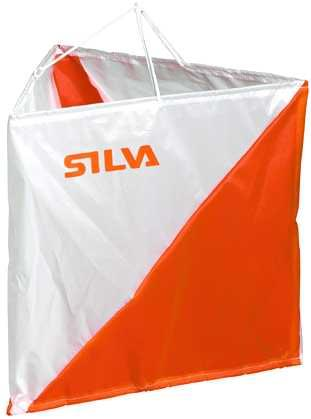
\includegraphics[width=.5\linewidth]{billeder/o-skaerm}
  \caption{Almindelig skærmpost}
  \label{fig:test1}
\end{minipage}%
\begin{minipage}{.5\textwidth}
  \centering
  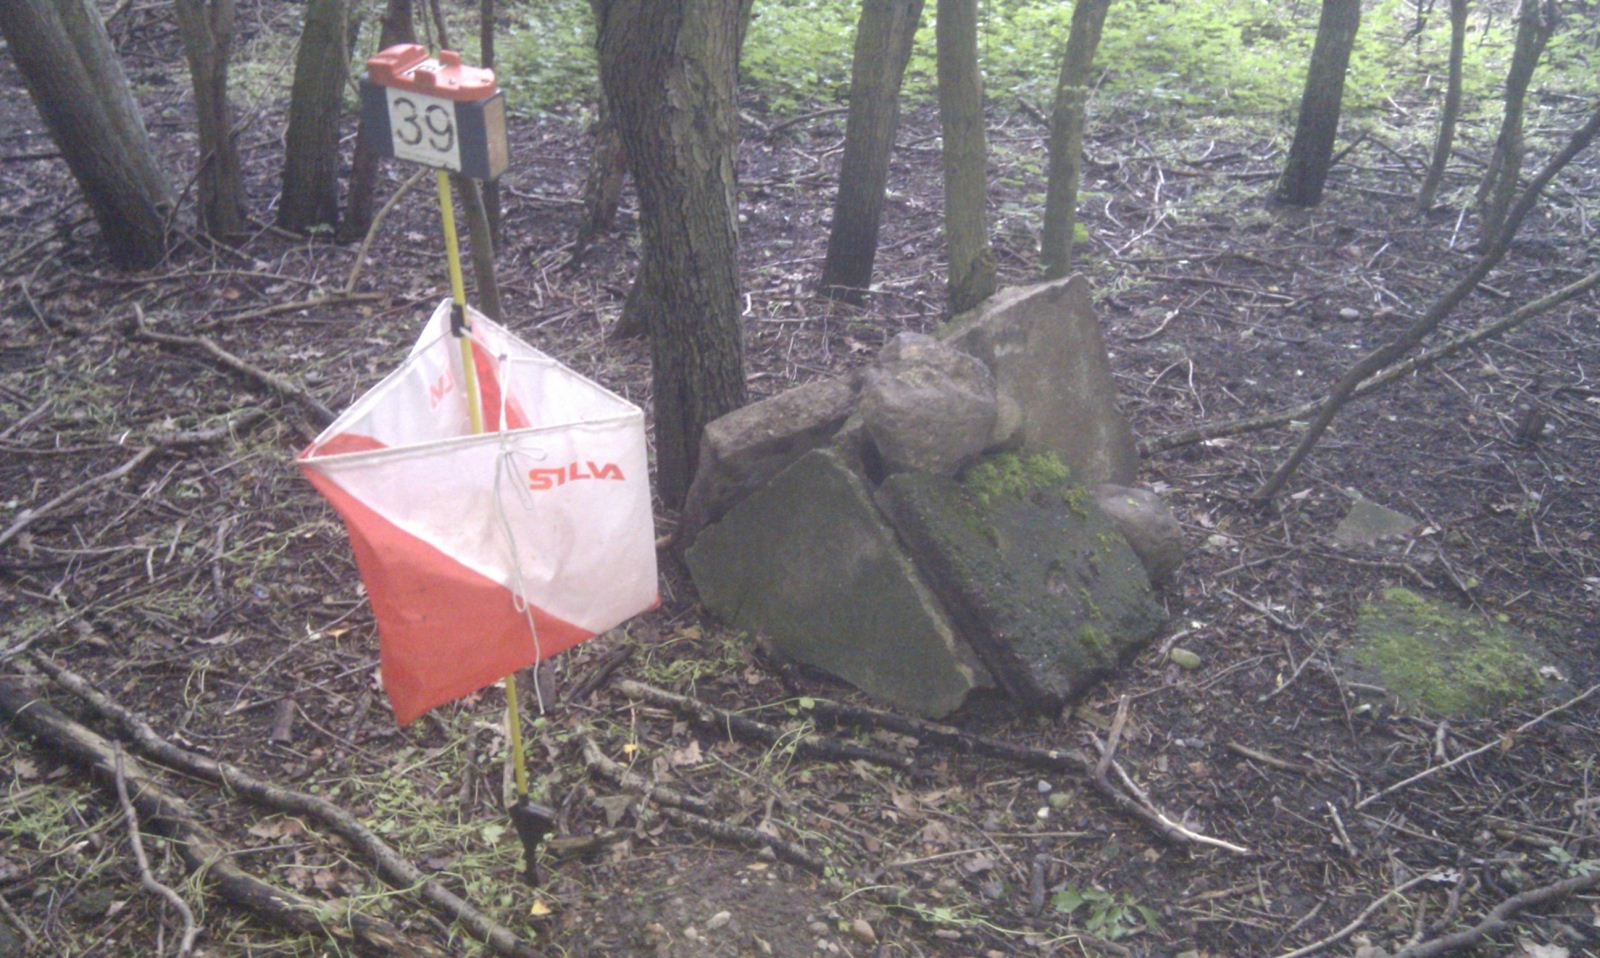
\includegraphics[width=1.0\linewidth]{billeder/banelaeggerkreativitet}
  \caption{Elektronisk post}
  \label{fig:test2}
\end{minipage}
\end{figure}

Der findes en række forskellige discipliner indenfor o-løb. Først er der Sprint, Mellem, Lang og  Ultralang, der er enkeltmandsløb, hvor den eneste forskel er distancen der løbes. Sprint er den korteste, og ofte afvikles i byer for at gøre det så simpelt og hurtigt som muligt, og Ultralang er den længste, hvor vindertiden typisk er højere end ved maratonløb. Udover standardløbene, findes også Nat, Stafet og Hold, der adskiller sig ved, som stafet og hold, at have flere løbere, eller ved natløb, ved at foregå om natten. 